\documentclass[11pt]{article}
\usepackage[a4paper, margin=2.54cm]{geometry}
\usepackage[utf8]{inputenc}
\usepackage[spanish, mexico]{babel}
\usepackage[spanish]{layout}
\usepackage[article]{ragged2e}
\usepackage{textcomp}
\usepackage{amsmath}
\usepackage{amssymb}
\usepackage{amsfonts}
\usepackage{enumerate}
\usepackage{graphicx}

% ============================================================================
% ============================================================================
% ============================================================================

\title{
  Entrega N° 2 \\
  \large Modelos Físicos
}
\author{
  Farizano, Juan Ignacio \\
  \and
  Mellino, Natalia \\
  \and
  Prato, Valentina
}
\date{}

% ============================================================================
% ============================================================================
% ============================================================================

\begin{document}

\maketitle
\noindent\rule{\textwidth}{1pt}

\section*{Ejercicio 12.14}

\subsubsection*{Enunciado}

Un tractocamión viaja a $60 mi/h$ cuando el conductor aplica los
frenos. Si se sabe que las fuerzas de frenado del tractor y el remolque son,
respectivamente, $3.600 lb$ y $13 700 lb$, determine:

\begin{enumerate}[a)]
  \item La distancia recorrida por el tractocamión antes de detenerse.
  \item La componente horizontal de la fuerza en el enganche entre el tractor
        y el remolque mientras éstos van frenando.
\end{enumerate}

\begin{figure}[h!]
  \begin{center}
    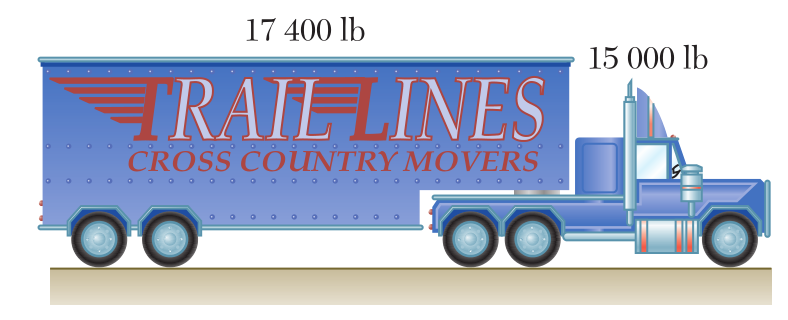
\includegraphics[width=0.75\linewidth]{ej14.png}
  \end{center}
\end{figure}

\subsection*{Resolución}

Por el enunciado sabemos que la velocidad inicial es $v_0 = 60mi/h = 88 ft/s$
y el peso del camión es igual a
$p = \underbrace{17400lb}_{p_1} + \underbrace{15000lb}_{p_2} = 32400lb$

Las fuerzas ejercidas por los frenos son:
\begin{align*}
  & F_1 = -13700lb \\
  & F_2 = -3600lb
\end{align*}

\subsection*{Apartado a)}

Por la segunda ley de Newton tenemos que $\sum F_x = ma$, luego:

\begin{align*}
  \sum F_x &= F_1 + F_2 = ma = \frac{p}{g} \\
           &\Rightarrow -13700lb - 3500lb = \frac{32400lb}{32.2 ft/s^2}a \\
           &\Rightarrow a = - \frac{17300lb \cdot 32.2ft/s^2}{32400lb} 
           = \underbrace{-17.19ft/s^2}_{\text{Desaceleración}}
\end{align*}

Usando la siguiente ecuación de movimiento uniformemente acelerado
\begin{align*}
  v^2 &= v^2_0 +2a(x-x_0) \rightarrow \text{buscamos distancia en} \; v = 0 \\
      &\Rightarrow 0ft^2/s^2 = 7744ft^2/s^2 - 34.38ft/s^2 \cdot \Delta x \\
      &\Rightarrow 34.38ft/s^2 \cdot \Delta x = 7744ft^2/s^2 \\
      &\Rightarrow \Delta x = 225.25ft
\end{align*}

\subsection*{Apartado b)}

La componente horizontal de la fuerza en el enganche es la fuerza que ejerce
el tractor sobre el remolque al tirarlo, la llamaremos T.
Nuevamente por segunda ley de Newton:
\begin{align*}
  \sum F_x &= T + F_1 = ma \\
           &\Rightarrow T = -F_1 + \frac{p_1}{g}a \\
           &\Rightarrow T = 13700lb - 17.19ft/s^2 \cdot \frac{17400lb}{32.2ft/s^2} \\
           &\Rightarrow T = 4411lb
\end{align*}

% ============================================================================

\section*{Ejercicio 12.25}

\subsection*{Enunciado}

Se aplica una fuerza constante \textbf{P} al pistón y a la varilla de masa total
$m$ para que se muevan en un cilindro lleno de aceite. Conforme se mueve el
pistón, se obliga a que el aceite atraviese los orificios en el pistón y ejerza
sobre este mismo una fuerza de magnitud $kv$ en la dirección opuesta al
movimiento del pistón. Si el pistón parte de reposo en t = 0 y x = 0, muestre
que la ecuación que relaciona a $x, v$ y $t$ es lineal en cada una de las
variables donde $x$ es la distancia recorrida por el pistón y $v$ es la rapidez
del mismo.

\begin{figure}[h!]
  \begin{center}
    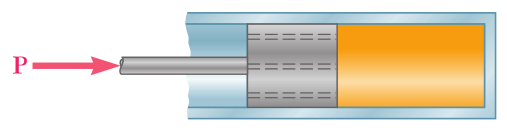
\includegraphics[width=0.75\linewidth]{ej25.png}
  \end{center}
\end{figure}

\subsection*{Resolución}

Por segunda ley de Newton tenemos que

\begin{align*}
  \sum F = ma &\Rightarrow P - kv = ma \\
  &\Rightarrow P - kv = m \frac{dv}{dt} \\ % recordemos que a = dv/dt
  &\Rightarrow \frac{1}{m}dt = \frac{1}{P - kv}dv \\
  &\Rightarrow \int_{0}^{t} \frac{1}{m}dt = \int_{0}^{v} \frac{1}{P - kv}dv \\ % despejamos v:
  &\Rightarrow \frac{t}{m} = -\frac{1}{k}(\ln{(P - kv)} - \ln{(P)}) \\
  &\Rightarrow t = -\frac{m}{k} \cdot \ln{\left(\frac{P - kv}{P}\right)} \\
  &\Rightarrow -\frac{k}{m}t = \ln{\left(\frac{P - kv}{P}\right)} \\
  &\Rightarrow \frac{P - kv}{P} = e^{-\frac{k}{m}t} \\
  &\Rightarrow P - kv = P \cdot e^{-\frac{k}{m}t} \\
  &\Rightarrow v = \frac{P}{k} - \frac{P}{k}e^{-\frac{k}{m}t} = \frac{dx}{dt} \\ %recordemos q v = dx/dt
  &\Rightarrow \int_{0}^{x} dx = \int_{0}^{t} \frac{p}{k} - \frac{p}{k} \cdot e^{\frac{-k}{m} t}dt \\
  &\Rightarrow x = \left. \frac{p}{k} \cdot t + \frac{pm}{k^2} \cdot e^{\frac{-k}{m}} \right\vert_0^t \\
  &\Rightarrow x = \frac{p}{k} \cdot t - m \cdot v % por lo tanto x es lineal
\end{align*}


\section*{Ejercicio 12.63}

\subsection*{Enunciado}

En el tubo de rayos catódicos que se muestra en la figura, los electrones 
emitidos por el cátodo y atraídos por el ánodo pasan a través de
un pequeño agujero en el ánodo, y luego viajan en línea recta con velocidad
v 0 hasta que inciden sobre la pantalla en A. Sin embargo, si se establece una
diferencia de potencial de $V$ entre las dos placas paralelas, los electrones 
estarán sujetos a una fuerza $F$ perpendicular a las placas mientras viajan entre
éstas, e incidirán en la pantalla en el punto B que está a una distancia $\delta$ 
de A. La magnitud de la fuerza $F$ es $F = eV/d$, donde $-e$ es la carga de un 
electrón y $d$ es la distancia entre las placas. Deduzca una expresión para la 
deflexión $\delta$ en términos de $V$, $v_0$ , la carga $-e$ y la masa $m$ de un 
electrón, así como las dimensiones $d$, $l$ y $L$.

\begin{figure}[h!]
  \begin{center}
    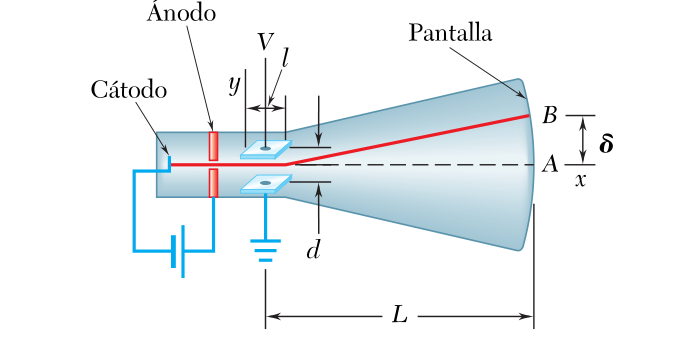
\includegraphics[width=0.75\linewidth]{ej63.png}
  \end{center}
\end{figure}


\subsection*{Resolución}

Fijamos nuestro sistema de referencia con $x$ positivo hacia la derecha, $y$
positivo hacia arriba y el origen situado en el borde izquierdo de las placas, a 
la misma altura del punto $A$. \\

Planteamos la Segunda Ley de Newton y despejamos la aceleración:

\begin{align*}
  \sum F &= m a \\
  \frac{e \cdot V}{d} &= m a \\
  a &= \frac{e \cdot V}{md}
\end{align*}

Tenemos dos tiempos: $t_1$ que representa el tiempo de viaje entre las placas y
$t_2$ que representa el tiempo de viaje restante hacia la pantalla. Como en
$t_0$ la partícula se encuentra en la posición (0, 0) podemos deducir:

\begin{align*}
  x_1 &= l = v_0 \cdot t_1 \Rightarrow t_1 = \frac{l}{v_0} \\
  x_2 &= L + \frac{1}{2}l \Rightarrow t_2 = \frac{l}{2v_0} + \frac{L}{v_0}
\end{align*}

Ahora, podemos deducir las posiciones $y_1$ e $y_2$ con respecto a los tiempos
obtenidos anteriormente.

\begin{equation*}
  y_1 = \frac{1}{2} \cdot \frac{eV}{md} \cdot t_1^2
\end{equation*}

\begin{align*}
  y_2 &= \delta = y_1 + v_1 (t_2 - t_1)  \\
      &= \frac{e v t_1^2}{2 m d} + \frac{e v t_1}{m d} (t_2 - t_1) \\
      &= \frac{e v t_1^2}{2 m d} + \frac{e v t_1 t_2}{m d} - \frac{e v t_1^2}{m d} \\
      &= \frac{e v t_1}{m d} (t_2 - \frac{t_1}{2}) \\
      &= \frac{e v l}{m d v_0} (\frac{L}{v_0}) \\
      &= \frac{e v l L}{m d v_0^2} \cdot
\end{align*}

\end{document}